\documentclass{beamer}
\usepackage[utf8]{inputenc}
\usepackage{graphicx}
\usepackage{amsmath}
\usepackage{amsfonts}
\usepackage{amssymb}
\usepackage{float}
\usepackage[verbose]{wrapfig}
\usepackage{textcomp}
\usepackage{color}

\newcommand{\argmax}{\operatornamewithlimits{argmax}}

\mode<presentation>
{
  \usetheme{Warsaw}
  \useinnertheme{circles}
  \usecolortheme{crane}

  \setbeamercovered{transparent}
  \beamertemplatenavigationsymbolsempty
  \useoutertheme{infolines}
}

\title[Spark Streaming] % (optional, use only with long paper titles)
{Spark Streaming}

\author [Kope{\'c}, Okulewicz]
{Mateusz Kope{\'c}, Micha{\l} Okulewicz}

\institute[ICS PAS]
{
Institute of Computer Science\\
Polish Academy of Sciences}

\date %[ ] % (optional, should be abbreviation of conference name)
{Big Data \\27 November 2014}

\subject{Real-time distributed computing}
%%%%%%%%%%%%%%%%%%%%%%%%%%%%%%%%%%%%%%%%%%%%%%%%%%%%%%%%%%%%%%%%%%%%%%%%
%%%%%%%%%%%%%%%%%%%%%%%%%%%%%%%%%%%%%%%%%%%%%%%%%%%%%%%%%%%%%%%%%%%%%%%%
\begin{document}

\begin{frame}
  \titlepage
\end{frame}

\begin{frame}
  \frametitle{Presentation Plan}
  \tableofcontents
  % You might wish to add the option [pausesections]
\end{frame}

%%%%%%%%%%%%%%%%%%%%%%%%%%%%%%%%%%%%%%%%%%%%%%%%%%%%%%%%%%%%%%%%%%%%%%%%
%%%%%%%%%%%%%%%%%%%%%%%%%%%%%%%%%%%%%%%%%%%%%%%%%%%%%%%%%%%%%%%%%%%%%%%%
\section{Spark}

\subsection*{Apache Spark\texttrademark}
\begin{frame}
\frametitle{What is Apache Spark\texttrademark?}

\begin{block}{Apache Spark\texttrademark}
\begin{itemize}
	\item distributed computations system
	\item not only MapReduce applications
	\item supports in-memory operations (Resilient Distributed Dataset)
	\item may use HDFS
\end{itemize}
\end{block}

\begin{block}{APIs}
\begin{itemize}
	\item Scala
	\item Java
	\item python
\end{itemize}
\end{block}

\end{frame}

%%%%%%%%%%%%%%%%%%%%%%%%%%%%%%%%%%%%%%%%%%%%%%%%%%%%%%%%%%%%%%%%%%%%%%%%
\begin{frame}
\frametitle{Spark architecture}
\begin{center}
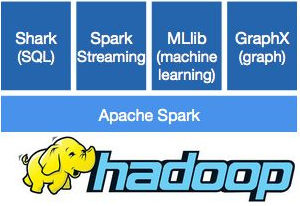
\includegraphics[height=0.4\textheight]{img/SparkHadoop.png}
\vspace{1em}
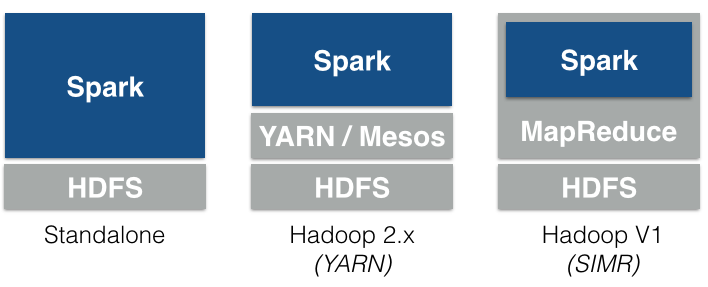
\includegraphics[height=0.4\textheight]{img/spark-on-hadoop.png}
\end{center}
\end{frame}

%%%%%%%%%%%%%%%%%%%%%%%%%%%%%%%%%%%%%%%%%%%%%%%%%%%%%%%%%%%%%%%%%%%%%%%%
%%%%%%%%%%%%%%%%%%%%%%%%%%%%%%%%%%%%%%%%%%%%%%%%%%%%%%%%%%%%%%%%%%%%%%%%
\section{Spark Streaming}

%%%%%%%%%%%%%%%%%%%%%%%%%%%%%%%%%%%%%%%%%%%%%%%%%%%%%%%%%%%%%%%%%%%%%%%%
\subsection*{Real-time computing}
\begin{frame}
\frametitle{Why do we want Spark Streaming?}
	\begin{itemize}
		\item Fraud detection
		\item Financial market analysis
		\item On-line surveillance
		\item Early earthquakes detection
		\item \ldots
	\end{itemize}
\end{frame}

%%%%%%%%%%%%%%%%%%%%%%%%%%%%%%%%%%%%%%%%%%%%%%%%%%%%%%%%%%%%%%%%%%%%%%%%
\begin{frame}
\frametitle{What is Spark Streaming?}

\begin{block}{Spark Streaming}
\begin{itemize}
	\item subproject of Apache Spark\texttrademark
	\item allows for real-time distributed stream processing
	\item utilizes an idea called Discretized Stream (DStream)
\end{itemize}
\vspace{-1em}
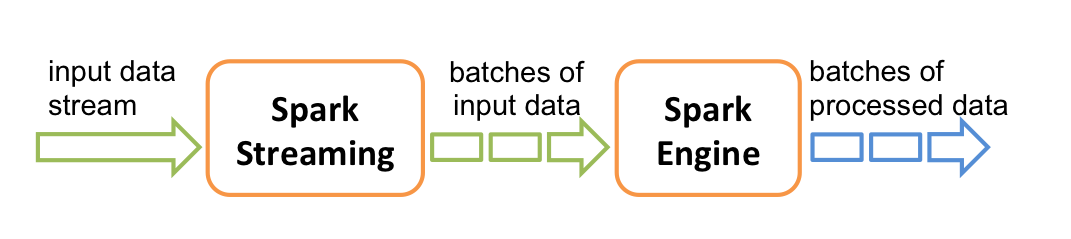
\includegraphics[width=\textwidth]{img/streaming-flow.png}
\vspace{-1em}
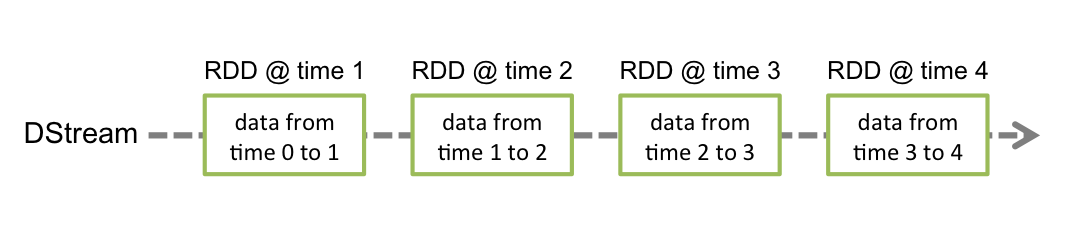
\includegraphics[width=\textwidth]{img/streaming-dstream.png}

\end{block}
\end{frame}

%%%%%%%%%%%%%%%%%%%%%%%%%%%%%%%%%%%%%%%%%%%%%%%%%%%%%%%%%%%%%%%%%%%%%%%%
%%%%%%%%%%%%%%%%%%%%%%%%%%%%%%%%%%%%%%%%%%%%%%%%%%%%%%%%%%%%%%%%%%%%%%%%
\section{Example 1: Stream processing task}
\begin{frame}
\frametitle{Example stream processing task}
\begin{block}{Data producer}
	Generates next integer every 100ms
\end{block}
\begin{block}{Data analyser}
	Counts all distinct numbers
\end{block}
\end{frame}

%%%%%%%%%%%%%%%%%%%%%%%%%%%%%%%%%%%%%%%%%%%%%%%%%%%%%%%%%%%%%%%%%%%%%%%%
\begin{frame}[allowframebreaks]
\frametitle{How to run Spark?}

\begin{block}{Running master on Linux}
	\begin{itemize}
		\item Run \texttt{sbin/start-master.sh}
		\item Check in browser if \texttt{http://localhost:8080} is available
	\end{itemize}
\end{block}

\begin{block}{Running worker on Linux}
	\begin{itemize}
		\item Get precompiled Spark 1.1.0 for Hadoop 1.x from \texttt{/home/2012/m.okulewicz/spark} and unpack it
		\item If necessary edit: \texttt{conf/spark-env.sh} and add location of~\texttt{JAVA\_HOME}
		\item Run \texttt{sbin/start-slave.sh 1 spark://phd01.phd.ipipan.waw.pl}
		\item Check in browser if \texttt{http://localhost:8081} is available and master points to \texttt{phd01.phd.ipipan.waw.pl}
	\end{itemize}
\end{block}
	
\begin{block}{Running task on Linux}
	\begin{itemize}
		\item Run: \\
		\texttt{./bin/spark-submit \\
  --class pl.waw.ipipan.phd.mkopec.sparkReceiver.SocketReceiver \\
  --master spark://phd01.phd.ipipan.waw.pl:7077 \\
  --executor-memory 20G \\
  --total-executor-cores 100 \\
  /path/to/jar.jar localhost 9999 1000 1}
	\end{itemize}
\end{block}

\end{frame}

%%%%%%%%%%%%%%%%%%%%%%%%%%%%%%%%%%%%%%%%%%%%%%%%%%%%%%%%%%%%%%%%%%%%%%%%
%%%%%%%%%%%%%%%%%%%%%%%%%%%%%%%%%%%%%%%%%%%%%%%%%%%%%%%%%%%%%%%%%%%%%%%%
\section{Example 2: Twitter}
\begin{frame}
\frametitle{Example stream processing task}
\begin{block}{Data producer}
	Retrieves stream of tweets containing specified keywords
\end{block}
\begin{block}{Data analyser}
	Counts most frequent words in tweets
\end{block}
\end{frame}

%%%%%%%%%%%%%%%%%%%%%%%%%%%%%%%%%%%%%%%%%%%%%%%%%%%%%%%%%%%%%%%%%%%%%%%%
\begin{frame}[allowframebreaks]
\frametitle{How to run Spark?}

\begin{block}{Running task on Linux}
	\begin{itemize}
		\item Run: \\
		\texttt{./bin/spark-submit \\
  --class pl.waw.ipipan.phd.mkopec.sparkReceiver.TwitterReceiver \\
  --master spark://phd01.phd.ipipan.waw.pl:7077 \\
  --executor-memory 20G \\
  --total-executor-cores 100 \\
  /path/to/jar.jar localhost 1000 1 polska,poland}
	\end{itemize}
\end{block}

\end{frame}

%%%%%%%%%%%%%%%%%%%%%%%%%%%%%%%%%%%%%%%%%%%%%%%%%%%%%%%%%%%%%%%%%%%%%%%%
%%%%%%%%%%%%%%%%%%%%%%%%%%%%%%%%%%%%%%%%%%%%%%%%%%%%%%%%%%%%%%%%%%%%%%%%
\begin{frame}[allowframebreaks]
	\frametitle<presentation>{Bibliography}
	\nocite{*}
	\bibliographystyle{plain}
	\tiny
	\bibliography{SparkStream}
\end{frame}

\end{document}


